\documentclass[]{article}
\usepackage[ngerman]{babel}
\usepackage{graphicx}
\usepackage{amsmath}
\usepackage[utf8]{inputenc}
\usepackage[T1]{fontenc}
\usepackage[ngerman]{babel}
\usepackage{courier}
\usepackage{hyperref} 
%opening
\title{Erfahrungen aus der Erstellung des Projektes \glqq ThermoAmpel\grqq{} für das Seminar \glqq Mikrocontrollerschaltungen - Realisierung in Hard- und Software\grqq}
\author{Ilhan Aydin, Lev Perschin}

\begin{document}

\maketitle
\newpage
\section{Einleitung}
\subsection{Erste Erfahrungen/Schritte}
Wir hatten wenig Vorwissen in diesem Bereich und haben noch nie einen Schaltplan erstellt, die Komponenten auf dem Board verteilt, es gedruckt, bestückt und anschließend programmiert. Das Wissen, welches wir hatten, waren Kenntnisse aus der Vorlesung "`Technische Informatik"' und ähnliche.
\subsection{Aufgabenstellung}
Die Aufgabe besteht daraus mittels eines Temperatur- und Luftfeuchtigkeitsensors die Temperatur und Luftfeuchtigkeit auszulesen und über die UART-Schnittstelle auszugeben. Zusätzlich lassen wir über die LEDs anzeigen, ob die Temperatur und Luftfeuchtigkeit im guten Bereich liegen.
\subsection{Hilfsmittel}
Als Hilfsmittel haben wir größtenteils das Datenblatt des Mikrocontrollers und die Datenblätter der eingebauten Komponenten verwendet. Zusätzlich haben wir die Seite \url{www.microchip.com/webdoc/avrassembler/avrassembler.wb_instruction_list.html} verwendet, welche die Instruktionen des Mikrocontrollers beschreibt. Weiterhin haben wir die Seite \url{www.mikrocontroller.net/} genutzt, die einige anschauliche Beispiele zu Assemblercode enthält. Abschließend hat der Leitfaden des Seminars uns bei der Vorgehensweise geholfen.
\section{Aufbau der Schaltung}
Dieser Abschnitt beschreibt unsere Herangehensweise an das Erstellen des Schaltplans. Dazu haben wir uns größtenteils an dem Leitfaden orientiert und die Aufgaben nacheinander realisiert. Zum Erstellen des Schaltplans haben wir EAGLE verwendet, da diese Software sich für Einsteiger empfiehlt.

\subsection{Schaltplan}
Für die Erzeugung des Schaltplans haben wir zunächst bei EAGLE den Mikrocontroller rausgesucht und nach und nach die benötigten Komponenten an den Mikrocontroller verbunden.
\subsubsection{Festspannungsregler}
Dazu gehörte erst einmal eine Spannungsversorgung. Für diese haben wir den Festspannungsregler \textit{7805TV} genutzt. 
In unserer Schaltung sollte der Festspannungsregler eine feste Ausgangsspannung liefern. Dazu wird dieser über jeweils einen Kondensator am Eingang und Ausgang verschaltet. Wie es genau verschaltet werden muss, kann man im Datenblatt nachschauen. 
Der Spannungsregler hat eine Ausgangsspannung von 5V, was ausreicht, um die ganze Platine mit Strom zu versorgen. Als Eingangsspannung legten wir eine Spannung von 10V fest. Hierbei ist zu beachten, dass die Differenz zwischen Eingangs- und Ausgangsspannung nicht zu groß sein sollte, da die Verlustleistung von der Differenz abhängt und somit größer wird.
\\Verbunden wird die Ausgangsspannung mit den Pins \texttt{AVCC} und \texttt{VCC} des Mikrocontrollers. Die Komponenten, die eine Versorgung benötigen, werden ebenfalls über die Ausgangsspannung versorgt.

\subsubsection{Takterzeugung}
Der Mikrocontroller hat für die Takterzeugung einen internen Oszillator. Man kann allerdings auch externe Oszillatoren verwenden. Der Mikrocontroller unterstützt laut Datenblatt folgende Arten: 
\begin{itemize}
\item External Crystal/Ceramic Resonator
\item External Low-frequence Crystal 
\item External RC Oscillator 
\item Calibrated Internal RC Oscillator
\item External Clock
\end{itemize}
Standardmäßig verwendet der Mikrocontroller seinen internen Oszillator, welche eine Frequenz von 1MHz hat. Um andere Oszillatoren zu verwenden, muss man die Fusebits entsprechend einstellen. Wir haben einen Quarz mit einer Frequenz von 4MHz verwendet. Dieser ist der Kategorie \textit{External Crystal/Ceramic Resonator} einzuordnen. In AtmelStudio wurde der Quarz des Mikrocontrollers beim Anschließen erkannt und die Fusebits automatisch gesetzt. 
\\Zum Verschalten des Quarzes benötigt man zwei Kondensatoren, um die Schwingsicherheit der Oszillatorschaltung zu gewährleisten. Die empfohlene Kapazität der Kondensatoren für den Quarz ist vom Hersteller festgelegt und ist im Datenblatt enthalten.
\\Verbunden wird der Quarz über die Pins \texttt{XTAL1} und \texttt{XTAL2}.

\subsubsection{ISP-Schnittstelle}
Die Verschaltung der ISP-Schnittstelle ist im Leitfaden vorgegeben. Wir haben die sechspolige Variante verwendet. Zur Verschaltung werden die Pins \texttt{MISO}, \texttt{SCK}, \texttt{MOSI}, \texttt{RESET} mit den entsprechenden Pins am Mikrocontroller verbunden. \texttt{$V_{CC}$} ist an den Ausgang des Festspannungsreglers angeschlossen und \texttt{GND} an Ground.

\subsubsection{Reset-Schaltung}
Die Verschaltung der Reset-Schaltung ist ebenfalls vorgegeben. Dafür verwendet man einen Taster, der über ein RC-Glied mit dem \texttt{RESET} Pin verbunden ist. Der Kondensator dient der hardwareseitigen Entprellung des Tasters. Bei einem Druck auf den Taster wird der Pin mit Ground verbunden. Das Signal fällt aufgrund des Kondensators nicht sprunghaft, sondern gedämpft auf den niedrigen Pegel. Weiteres zur Entprellung bei \ref{interrupts}.

\subsubsection{LEDs}
Für die Verschaltung der LEDs haben wir drei Pins aus Port A verwendet. Dabei ist es wichtig, Vorwiderstände vorzuschalten. Der Wert des Widerstands berechnet sich aus folgender Formel:
\begin{equation*}
R = \frac{U_R}{I}\text{,}
\end{equation*}
wobei $U_R$ sich aus der Differenz zwischen der Spannung, die aus dem Pin kommt, welche bei uns 5V entspricht, und der Durchlassspannung der LED, die wir als 2V angenommen haben, ergibt. Den Strom $I$ haben wir auf 20mA begrenzt, da ein Pin des Mikrocontrollers laut Datenblatt maximal 40mA aufnehmen darf. Damit ergibt sich ein Widerstand von 150$\Omega$.

\subsubsection{Taster für Interrupts}
Zum Auslösen von externen Interrupts haben wir drei Taster an die Pins \texttt{INT0}, \texttt{INT1} und \texttt{INT2} angeschlossen. Damit eine fallende Flanke einen Interrupt auslöst, muss auf Druck des Tasters das Signal auf einen niedrigen Pegel fallen. Dazu sind die Taster am anderen Ende lediglich mit Ground verbunden. Das bedeutet allerdings, dass wir eine Softwarelösung für die Entprellung der Tasten implementieren müssen.
\\Im Programm des Mikrocontrollers kann man durch das Setzen von Bits im entsprechenden Register festlegen, ob eine fallende oder eine steigende Flanke ein Interrupt auslösen soll. Dazu mehr im Abschnitt \ref{interrupts}.

\subsubsection{A/D-Wandlung}
Die Verschaltung des A/D-Wandlers haben wir nach einer Application Note von Atmel eingebaut. Dazu verbinden wir \texttt{AREF} über ein RC-Glied mit einem Pin aus Port A. Laut Application Note sollte bei einer Zählfrequenz von 4Mhz der Widerstand 30k$\Omega$ betragen und der Kondensator 8.2nF.
Die Spannung, die wir umwandeln wollen, soll einstellbar sein. Die wird durch einen Potentiometer geregelt, der an einen anderen Pin von Port A angeschlossen ist. Dieser Potentiometer wird über die Ausgangsspannung des Festspannungsreglers versorgt. 

\subsubsection{UART-Schnittstelle}
Für die UART-Schnittstelle haben wir eine vier-polige Molex Stiftleiste verwendet. Dabei haben wir den ersten Pin an die Spannung des Festspannungsreglers, den zweiten Pin an \texttt{RXD}, den dritten Pin an \texttt{TXD} und den vierten Pin an Ground angeschlossen.

\subsubsection{Zusätzliches}
Die offenen Pins des Mikrocontrollers haben wir mit Stiftleisten bzw. Stiften versehen. Dadurch kann man sie später nach Bedarf verwenden.
\\Beim Erstellen des Schaltplans sollte man darauf achten, dass es so übersichtlich wie möglich bleibt. Dazu kann man beispielsweise die Komponenten, die gemeinsam eine Funktionalität zur Verfügung stellen, gruppiert darstellen.

\subsection{Aufbau des Boards}
\subsubsection{Anordnung der Komponenten}
Für die Anordnung der Komponenten war es uns wichtig, so wenig Platz wie möglich zu verbrauchen. Dazu haben wir zum einen Komponenten gleicher Art örtlich gruppiert, zum anderen nach Funktionalität. Beispielsweise haben wir die Taster für die externen Interrupts gruppiert, während wir den Taster für den Reset an eine andere Stelle platziert haben. Auch wollten wir, dass die Anordnung der LEDs eine Ampel darstellt. Dementsprechend haben wir sie gruppiert positioniert.
\\Generell hat man bei der Anordnung der Komponenten viel Freiraum.

\subsubsection{Erstellung von Groundplane}
Alle Pins, die in unserem Schaltplan mit Ground verbunden waren, wollen wir mit der Groundplane verbinden. Für die Erstellung des Groundplanes haben wir uns an die Anleitung der Seite \url{https://www.build-electronic-circuits.com/eagle-ground-plane/} gehalten. Diese beschreibt das Erstellen der Groundplane in drei Schritten.

\subsubsection{Erstellung von Leitungen}
Um die Leitungen in EAGLE nicht manuell zeichnen zu müssen, bietet die Software einen "`Autorouter"' an. Diesen haben wir verwendet und waren mit dem Ergebnis zufrieden. Falls man nicht zufrieden sein sollte, kann man die Leitungen auch danach manuell ändern.
\\Bei den Leitungen ist es wichtig, dass diese nicht in einem 90$^\circ$ Winkel verlaufen. Ebenfalls wichtig ist die Breite der Versorgungsleitung, welche eine gewisse Breite haben sollte, damit kein zu hoher Widerstand in der Versorgungsleitung entsteht. In EAGLE bilden die Versorgungsleitungen ein Netz und für dieses Netz kann man die Breite einstellen. Dort haben wir dann eine Breite von 1mm eingestellt.



\section{Funktionsweise der Software}
Dieser Abschnitt beschreibt unsere Herangehensweise an das Programmieren des Mikrocontrollers und die Funktionsweise des Programms. Ausgehend davon, dass in der Platine alles korrekt verschaltet ist, kann man mit dem Programmieren beginnen. Wir haben dafür einen Programmer von DIAMEX verwendet. Vorteil bei diesem Programmer ist, dass es die Platine mit 5V versorgen kann, sodass man beim Programmieren die Platine nicht extra an eine Stromversorgung anschließen muss. 
Zum Testen, ob der Mikrocontroller mit unserem Programm überschrieben worden ist, haben wir vorerst ein einfaches Programm geschrieben, welches die LEDs ansteuert. Nachdem der Mikrocontroller das LED-Programm richtig ausgeführt hat, begannen wir mit der Implementation unserer Aufgabe.
\subsection{Aufbau des Programms}
In diesem Abschnitt wird der Aufbau des Programms beschrieben.
\\Vor allem Anderen sollte man "`m16adef.inc"' über \texttt{.include} einbinden, damit man für den Mikrocontroller spezifische Definitionen verwenden kann. Danach sollte man um das Programm lesbarer zu machen, häufig verwendete Register oder Register, die nur einen bestimmten Zweck haben, über \texttt{.def} Namen geben. Ebenfalls nützlich ist auch die Verwendung von \texttt{.equ}, womit man häufig verwendeten Werten Namen geben kann.
\\Durch \texttt{.cseg} gibt man an, dass man sich ab der Zeile im Codesegment befindet. Als Erstes sollte hier die Startadresse stehen. Zu dieser sollte man beim Start oder Reset des Mikrocontrollers springen. Dies erreicht man mit \texttt{.org} für die Adresse 0x000. Dort gibt man dann an, wo das Programm beginnen soll.
\\Bevor es in die Hauptroutine geht, legen wir fest, was beim Starten oder Neustarten des Mikrocontrollers passieren soll. Zunächst wird der Stack initialisiert. Danach legen wir die LED Pins als Ausgang fest. Weiterhin aktivieren und konfigurieren wir hier die Interrupts. Zudem wollen wir den 8-Bit und 16-Bit Timer verwenden, welche hier ebenfalls konfiguriert werden. Zum Schluss initialisieren wir noch die UART Schnittstelle.
\\Die Hauptroutine ist eine Endlosschleife und besteht aus der ständigen Abfrage der Temperatur und relativen Luftfeuchtigkeit gekoppelt mit einem kleinen Wetterbericht, welcher die abgefragten Werte über die UART Schnittstelle überträgt. Zwischen jeder Abfrage gibt es einen Delay von einer Sekunde, damit der Sensor nicht überbelastet wird.

\subsection{Timer/Counter}
Wir benötigen den Timer, um Verzögerungen in unserem Programm verwenden zu können. Der Timer im Mikrocontroller ist ein Register, welches in jedem Takt inkrementiert wird. Der verwendete Quarz schwingt mit 4MHz, was bedeutet, dass ein Takt 250ns dauert. Ein 8-Bit Timer würde bei dieser Geschwindigkeit für das Zählen von 0 bis 255 $250ns*255 = 63750ns = 63,75\mu s$ brauchen, während ein 16-Bit Timer  $250ns*65535 = 16383750ns = 16,38ms$. Für unser Programm wollen wir eine Routine implementieren, die ungefähr 500ms dauert. Dazu könnten wir den 16-Bit Timer 31 Mal durchlaufen lassen. Wir könnten aber auch einstellen, dass der Timer nicht in jedem Takt inkrementiert werden soll, was wir dann auch gemacht haben. Dies macht man über den Prescaler. Um den Prescaler des 16-Bit Timers auf 64 zu setzen, also den Timer alle 64 Takte inkrementieren zu lassen, setzen wir die Bits \texttt{CS11} und \texttt{CS10} im Register \texttt{TCCR1B} auf 1. Zusätzlich setzen wir im selben Register das Bit \texttt{WGM12} auf 1. Dadurch operiert der Timer im Clear Timer on Compare match (CTC) Modus, was bewirkt, dass der Timer beim Erreichen des Wertes, der im Register \texttt{OCR1A} bzw. den Registern \texttt{OCR1AH} und \texttt{OCR1AL} festgelegt ist, zurückgesetzt wird. 
\\Für unsere Routine berechnen wir zunächst, bei welchem Wert 500ms vergangen sind. Dazu lösen wir die Gleichung $\frac{1}{4000000/64} * x = 0.5$ nach x auf und erhalten damit den Wert 31250. Das bedeutet, es braucht 31250 Takte, damit bei einer Taktrate von 4MHz und verwendetem Prescaler von 64 500ms vergehen. Die acht höherwertigen Bits des Wertes laden wir in \texttt{OCR1AH} und die acht niederwertigen in \texttt{OCR1AL}. 
\\Dann setzen wir den Counter vom Timer auf 0. Wichtig ist, dass das Schreiben des Counters atomar geschehen muss und außerdem die höherwertigen Bits zuerst geschrieben werden müssen. Für die Atomarität deaktivieren wir globale Interrupts und aktivieren sie wieder nach dem Schreiben. Der Counter befindet sich in den Registern \texttt{TCNT1H} und \texttt{TCNT1L}.
\\Nachdem der Counter auf 0 gesetzt ist, warten wir in einer Schleife bis das \texttt{OCF1A} Bit im \texttt{TIFR} gesetzt ist. Ist das Bit gesetzt, bedeutet es, dass der Counter den Wert im \texttt{OCR1A} Register angenommen hat und somit 500ms vergangen sind. Danach setzen wir \texttt{OCF1A} zurück, indem wir dort eine 1 schreiben.
\\Um im unserem Programm nun eine Verzögerung von einer Sekunde zu benutzen, führen wir diese Routine zwei mal aus. Für kürzere Verzögerungen verwenden wir Routinen, die andere Werte in das Register \texttt{OCR1A} schreiben.


\subsection{Interrupts}
\label{interrupts}
Für die Aktivierung von globalen Interrupts setzt man zunächst das \texttt{I} Bit im \texttt{SREG} Register. Der Befehl \texttt{sei} macht genau dies. Um die Interrupts bei den Pins \texttt{INT0}, \texttt{INT1} und \texttt{INT2} nun zu aktivieren, setzen wir im \texttt{GICR} Register die Bits \texttt{INT0}, \texttt{INT1} und \texttt{INT2} auf 1. Damit ein Interrupt beim Drücken des Knopfes erzeugt wird, muss eingestellt werden, dass ein Interrupt für \texttt{INT0-INT2} bei einer fallenden Flanke erzeugt wird. Dies stellt man im \texttt{MCUCR} Register ein, indem man für \texttt{INT0} das Bit \texttt{ISC01} und für \texttt{INT1} das Bit \texttt{ISC11} auf 1 setzt. Für \texttt{INT2} werden standardmäßig Interrupts bei einer fallenden Flanke erzeugt. Um jetzt auf Interrupts zu warten, setzt man die Pins \texttt{INT0}, \texttt{INT1}, \texttt{INT2} auf Eingang und legt eine 1 an. 
\\Die Behandlung eines Interrupts kann man mittels \texttt{.org} realisieren. Dazu muss man die Programmadresse kennen, auf die bei den Interrupts gesprungen wird. Beispielsweise wird bei einem Interrupt am Pin \texttt{INT0} auf die Adresse \texttt{0x002} gesprungen. Dort kann man dann festlegen, dass beim Interrupt auf eine beliebige Routine gesprungen wird. Abbildung 1 zeigt, wie wir die Interrupts implementiert haben.
\begin{figure}[h]
	\centering
	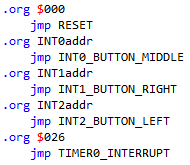
\includegraphics[width=0.35\columnwidth]{Interrupt.png}
	\caption{Interrupt}
\end{figure}
\\Der Code bewirkt, dass bei einem Interrupt am Pin \texttt{INT0} auf die Routine \texttt{INT0\_BUTTON\_MIDDLE} gesprungen wird.
\\Die Adressen für die Interrupts, die man \texttt{.org} mitgeben muss, findet man im Datenblatt des Mikrocontrollers. Wichtig bei der Verwendung von \texttt{.org} ist, dass man die mitgegebenen Adressen in aufsteigender Reihenfolge implementieren muss. Dabei kann man auch Definitionen wie \texttt{INT0addr} verwenden, welche im "`m16adef.inc"' festgelegt wurden.
\\Ebenfalls wichtig zu beachten ist, dass aufgrund des Prellens eines Tasters bei einem Tastendruck sehr viele Interrupts erzeugt werden. Um zu verhindern, dass die Routine bei einem Tastendruck nicht mehr als einmal ausgeführt wird, kann eine Entprellung über Software oder Hardware erfolgen. 
\\Wir entprellen über Software. Dazu deaktivieren wir bei einem Interrupt an einem Pin alle Interrupts für diesen Pin, damit die Routine auch wirklich nur einmal ausgeführt wird. Bei uns ist die Reaktivierung nicht implementiert, da es zu einem nicht vorhergesehenen Verhalten führt. Wenn man es wieder aktivieren möchte, müsste man es wie folgt machen: Man setzt einen Timer auf 0. Den Timer benutzt man, um die Interrupts für den Pin unabhängig von der Routine nach 10ms wieder zu aktivieren. Die Zeit, die man warten sollte, hängt von dem Knopf ab, den man benutzt. Unser Knopf prellt laut Datenblatt ungefähr 5ms lang. Sicherheitshalber würden wir mit dem Aktivieren doppelt so lange warten. Wichtig ist auch, dass man nicht in der Routine selbst warten sollte, da das den ganzen Programmfluss blockiert. 
\\Man kann auch entprellen, indem man das Signal am Pin mehrfach ausliest und erst, wenn das Signal stabil ist, die Aktion für den Interrupt durchführen. Stabiles Signal bedeutet hier, dass man mehrfach den selben Wert beim Lesen des Pins erhält. Vorteil an dieser Lösung ist, dass ein kurzer versehentlich hergestellter Kontakt keine Aktion ausführt.
\\Durch zusätzliche Hardware kann man ebenfalls entprellen. Eine kostengünstige Lösung ist die Verwendung von einem RC-Glied, damit der Wechsel des Pegels nicht sprunghaft geschieht. Eine andere Lösung wäre die Verwendung von prellfreien Schaltern. Nachteil an dieser Lösung ist, dass solche Schalter teuer sind und man auch nicht sicher sein kann, dass diese Schalter nach einiger Zeit immer noch gut funktionieren. Heißt also, dass sie nach gewisser Zeit anfangen könnten, zu prellen.
\\Die bessere Lösung hängt von der Anwendung und vom Budget ab. 
\\Wenn beispielsweise die Platine keinen Raum für zusätzliche Hardware bietet, eignet sich eine Softwarelösung. Möchte man, dass nicht jedes kurz auftauchende Signal ein Interrupt erzeugt, kann man das ebenfalls über Software regulieren. 
\\Eine Hardwarelösung würde sich empfehlen, wenn man beispielsweise die Interruptroutinen so kurz wie möglich halten will. 

\subsection{Ansteuern des Sensors}
\subsubsection{Wie man es nicht machen sollte}
Zunächst haben wir probiert, mit dem Sensor über das Two-wire Serial Interface (TWI) zu kommunizieren. Wie man über TWI kommuniziert ist im Datenblatt des AtMega16A ausführlich mit Codebeispielen beschrieben. Nach der Implementierung einer Routine zum Kommunizieren über TWI fiel uns auf, dass der Sensor TWI gar nicht unterstützt. Eine andere Lösung musste her.
\subsubsection{Wie man es machen sollte}
Wie man mit dem Sensor richtig kommuniziert, steht im Datenblatt des Sensors geschrieben. Dazu sendet man dem Sensor ein Kommando über den \texttt{SCK} und \texttt{DATA} Pin des Sensors, wartet auf die Bearbeitung des Kommandos und liest zum Schluss die Antwort aus. 
Das Senden eines Kommandos wird mit über das Senden der folgenden Bitfolge initiiert, welche im Datenblatt auch "`Transmission Start"' genannt wird: 
\begin{figure}[h]
	\centering
	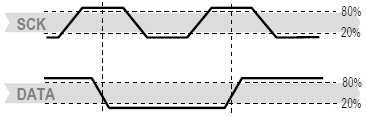
\includegraphics[width=0.5\columnwidth]{transmission_start.png}
	\caption{Transmission Start}
\end{figure}
\\ Um das Senden im Programm zu realisieren, setzt man zunächst die Pins, über die \texttt{SCK} und \texttt{DATA} verbunden sind, auf Ausgang. Dann legt man bei \texttt{DATA} eine 1 und bei \texttt{SCK} eine 0 an, damit der Zustand von \texttt{DATA} mit High und der von \texttt{SCK} mit Low beginnt, wie auch in Abbildung 2 dargestellt ist. Wie man weiter vorgeht, kann man der Abbildung entnehmen. Wenn der Zustand vom \texttt{SCK} oder \texttt{DATA} von Low auf High wechselt, bedeutet das, dass man an den mit \texttt{SCK} oder \texttt{DATA} verbundenen Port eine 1 anlegt. Der Wechsel von High zu Low entspricht dem anlegen einer 0. Nachdem man Transmission Start übertragen hat, kann man nun ein Kommando übertragen. Um beispielsweise die Temperatur abzufragen, sendet man die Sequenz 00000011. Das Senden geschieht ebenfalls durch das Setzen und Entfernen von Bits am Port von \texttt{SCK} und \texttt{DATA}. Wenn der Sensor ein Kommando erhalten hat, sendet er ein ACK zurück. Zum Überprüfen, ob das Senden des Kommandos erfolgreich war, setzt man \texttt{DATA} auf Eingang und legt eine 1 an, um den internen Pullup-Widerstand zu nutzen. Dies ist nötig, um die vom Sensor gesendeten Bits lesen zu können. Wird \texttt{DATA} vom Sensor aus auf Low gesetzt, hat er das Kommando erhalten. Nun wartet man bis die Messung fertig ist. Der Sensor setzt \texttt{DATA} auf Low, wenn er die Messung beendet hat. Das Lesen der Daten erfolgt byteweise. Nachdem man ein Byte gelesen hat, sendet man dem Sensor ein ACK und liest danach das nächste Byte aus. Falls die Daten keine höhere Genauigkeit als acht Bit haben, ist dieses Byte 0. Insgesamt liest man drei Bytes aus, wobei das letzte Byte die Checksumme beinhaltet. Die Kommunikation endet nach dem Auslesen des dritten Bytes. Man kann sie auch nach dem Lesen des zweiten Bytes beenden, wenn man die Checksumme nicht benötigt. Dazu lässt man \texttt{DATA} nach dem Senden des ACKs auf High. 
\\Beim Kommunizieren ist es wichtig, nicht zu vergessen, dass wenn man etwas senden will, der Port von \texttt{DATA} auf Ausgang und beim Lesen auf Eingang gesetzt werden muss. Zudem sollte man die Häufigkeit der Anfragen auf eine pro Sekunde beschränken, um die vom Sensor abgegebene Wärme zu reduzieren.
\\Wichtig ist auch, dass der Sensor nach dem Starten des Mikrocontrollers oder nach dem Senden eines Softresetkommandos an den Sensor 11ms braucht, damit er richtig funktioniert.
\\Da wir nun die Routine zum Abfragen des Sensors haben, können wir die relative Luftfeuchtigkeit und die Temperatur abwechselnd messen. Damit wir die selbe Routine nicht zwei mal implementieren müssen, geben wir in einem Register das Kommando an, welches gesendet werden soll und rufen dann die Routine auf.

\subsection{Auswerten der Daten}
Die Daten, die man vom Sensor erhält, müssen für die Ausgabe umgerechnet werden. Dazu gibt es im Datenblatt des Sensors Formeln, wie zum Beispiel folgende für die Berechnung der relativen Luftfeuchtigkeit:
\begin{equation*}
RH_{linear} = c_1 + c_2*SO_{RH} + c_3*SO_{RH}^{2} \left(\%RH\right)\textbf{,}
\end{equation*}
wobei $SO_{RH}$ die vom Sensor ausgelesenen Bits bezeichnet. Wenn $SO_{RH}$ eine Genauigkeit von 12 Bit hat, verwendet man für die Konstanten $c_1$, $c_2$ und $c_3$ folgende Werte: $c_1 = -2.0468$, $c_2 = 0.0367$, $c_3 = -1.5955*10^{-6}$.
Beispielsweise würde die vom Sensor erhaltene Bitfolge \texttt{0000 0100 0011 0001} (1073) einer relativen Luftfeuchtigkeit von 35.50\% entsprechen.\\
Die Formel kann man allerdings nicht im Mikrocontroller ohne Weiteres verwenden, da diese Genauigkeiten zum Berechnen erfordert, die der Mikrocontroller nicht aufbringt. Eine Möglichkeit zum Umwandeln der Bits in relative Luftfeuchtigkeit oder Temperatur besteht daraus, die entsprechenden Werte für die relative Luftfeuchtigkeit und die Temperatur für alle Bits vorher auszurechnen und in Form einer Lookup-Tabelle im Programm zu realisieren, damit der Mikrocontroller keine aufwändigen Rechnungen machen muss. Man bräuchte also bei einer Messung mit einer Genauigkeit von 14 Bit eine Lookup-Tabelle mit $2^{14}-1 = 16383$ Einträgen. Um die Einträge zu reduzieren, haben wir die Genauigkeit der Messungen durch mehrfache Division durch zwei auf acht Bit reduziert. Dafür braucht man nun eine Tabelle mit $2^8-1 = 255$ Einträgen. Realisiert wird das nun über das \texttt{DB}-Directive, was für die relative Luftfeuchtigkeit wie in Abbildung 3 aussehen kann.
\begin{figure}[h]
	\centering
	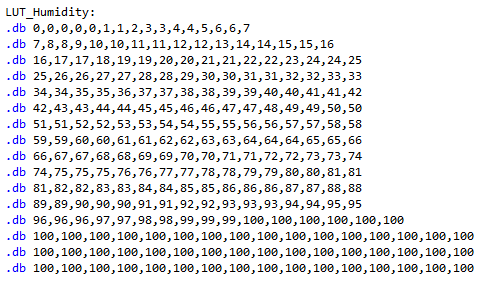
\includegraphics[width=0.8\columnwidth]{LUT.png}
	\caption{Lookup-Tabelle für relative Luftfeuchtigkeit}
\end{figure}
\\
Die erhaltenen Bits kann man jetzt als Index für den entsprechenden Wert der Bitfolge benutzen. Beispielsweise würde jetzt der Wert 1073, welcher mit einer Genauigkeit von 12 Bit gemessen wurde, durch 16 geteilt und als Index verwendet werden (1073/16 = 67). Der 67. Eintrag der Tabelle entspricht dem Wert 35\% (zuvor 35.50\%). Den Verlust der Genauigkeit nehmen wir hier für eine einfache Implementierung in Kauf. Der Zugriff auf den Eintrag erfolgt über den Befehl \texttt{lpm}. Dazu wird zunächst die Adresse der Tabelle, um eine Stelle nach links verschoben, in den Z Pointer geladen und der Index auf die Adresse addiert, um beim Verwenden von \texttt{lpm} den richtigen Eintrag zu laden.

\subsection{Ausgabe über UART}
Vor dem Benutzen der UART Schnittstelle muss man sie richtig initialisieren. Dazu schreibt man zunächst in das \texttt{UBRRH} und \texttt{UBRRH} Register einen Wert, der abhängig von der Baudrate und der Frequenz des verwendeten Quarz' ist, wobei in das \texttt{UBRRH} Register die acht höherwertigen und in das \texttt{UBRRH} die acht niederwertigen Bits des Wertes stehen müssen. Der Wert wird für den asynchronen normalen Modus, welchen wir verwendet haben, mit folgender Formel berechnet:
\begin{equation*}
UBRR = \frac{f_{OSC}}{16*BAUD} -1
\end{equation*}
\\Bei einer Frequenz von 4MHz und einer Baudrate von 9600 entspricht das dem Wert 25. \\Zusätzlich muss man den Signalaufbau festlegen. Um einen 8N1 Aufbau zu haben, also einen Aufbau, welcher aus acht Datenbits, keine Paritätsbits und einem Stoppbit besteht, muss man im \texttt{UCSRC} Register die Bits in den Feldern \texttt{URSEL}, \texttt{UCSZ1} und \texttt{UCSZ0} auf 1 und die Felder \texttt{UPM1}, \texttt{UPM0} und \texttt{USBS} auf 0 setzen. Dabei erlaubt \texttt{URSEL} das Schreiben in das \texttt{UCSRC} Register, \texttt{UCSZ1} und \texttt{UCSZ0} bestimmen die Anzahl der Datenbits, \texttt{UPM1} und \texttt{UPM0} bestimmen den Paritätsmodus und \texttt{USBS} die Anzahl der Stopbits. Standardmäßig sind alle Felder für unseren gewünschten Signalaufbau entsprechend gesetzt. 
\\Um vom Mikrocontroller aus etwas Senden zu können, muss jetzt nur noch der Transmitter aktiviert werden. Dazu setzt man im \texttt{UCSRB} Register das \texttt{TXEN} Bit auf 1.
\\Um zu wissen, ob der Mikrocontroller bereit zum Senden ist, überprüft man das \texttt{UDRE} Bit im \texttt{UCSRA} Register. Ist das Bit gesetzt, bedeutet das, dass man ein Byte in das \texttt{UDR} Register laden und senden kann. Das \texttt{UDRE} Bit gibt hierbei lediglich an, ob das \texttt{UDR} Register leer und bereit für den Empfang von neuen Daten ist. Das Senden kann jetzt wie in Abbildung 4 aussehen.
\begin{figure}[h]
	\centering
	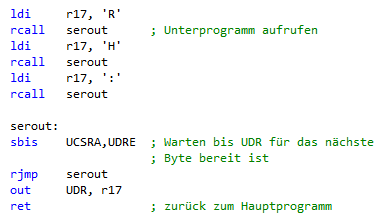
\includegraphics[width=0.7\columnwidth]{UART.png}
	\caption{Übertragung von "`RH:"'}
\end{figure}
\\Die gesendeten Werte werden als ASCII Werte interpretiert und dargestellt. Das bedeutet, dass man die Temperatur oder die relative Luftfeuchtigkeit in ASCII korrekt umwandeln muss, damit sie richtig dargestellt werden. Für dreistellige Zahlen benötigt man dafür drei Register. Möchte man beispielsweise die Zahl 123 übertragen, sendet man nacheinander die ASCII Symbole '1', '2', '3'. Für die Umwandlung verwenden wir eine Routine aus dem Internet, die binäre Zahlen in ASCII Werte umwandelt. Im Grunde zählt diese Routine die Hunderter, Zehner und Einer der Zahl und benutzt das Symbol '0' als Offset, um die Hunderter, Zehner und Einer jeweils als Symbol darzustellen.
\\Zu dem Umwandeln muss man noch beachten, dass auch negative Temperaturen richtig angezeigt werden muss. Da der Sensor eine maximale Temperatur von 123,8$^\circ$C messen kann, also alle positiven Temperaturen mit sieben Bits darstellen kann, behandeln wir das MSB als Vorzeichen Bit, wobei die restlichen Bits in ASCII Symbole umgewandelt werden sollen. Anhand des MSB können wir nun '+' für positive und '-' für negative Temperaturen mit angeben.

\subsection{Anzeige über die LEDs}
Wir verwenden die LEDs um anzuzeigen, ob die relative Luftfeuchtigkeit und die Temperatur im guten Bereich liegen. Ist die relative Luftfeuchtigkeit im schlechten Bereich, leuchtet die rote LED. Ist die Temperatur im schlechten Bereich, leuchtet die gelbe LED. Nur wenn beide Werte im guten Bereich sind, leuchtet die grüne LED. Für die relative Luftfeuchtigkeit haben wir Werte von 40\%-60\% und für die Temperatur 20$^\circ$C-25$^\circ$C als guten Bereich festgelegt.
\\Da man die Werte schon umgewandelt vorliegen hat, kann man das ganze über einige Vergleiche realisieren.


\subsection{Debug/Simulation}
Der Debugger im AtmelStudio war nur bedingt hilfreich, da wir ihn nicht nutzen konnten, während der Mikrocontroller ausgewählt war. Wir konnten einen simulierten Mikrocontroller auswählen und so den Debugger benutzen. Um zu testen, ob beispielsweise die Kommunikation mit dem Sensor funktioniert, genügte das allerdings nicht. Man kann auch über eine Stimuli-Datei eingehende Signale simulieren. Jedoch wäre es zu aufwändig, die Kommunikation mit dem Sensor damit zu simulieren. \\Stattdessen haben wir die LEDs verwendet, um zu schauen, ob unser Code eine Routine vernünftig ausführt. Damit konnten wir höchstens Fehler einschränken, allerdings nicht die Werte, die zu einem Fehler führten, überprüfen. \\Einige Fehler, die unabhängig von eingehenden Signalen vorhanden waren, konnten wir auch durch den simulierten Mikrocontroller ermitteln, da man dort beim Debuggen die Werte im Speicher anschauen kann. Also kann dieser in manchen Fällen nützlich sein.

\section{Schwierigkeiten}
Bei dem Projekt hatten wir mit einigen Schwierigkeiten zu tun. Im Folgenden listen wir einige davon auf, wobei wir auch den Lösungsansatz mitgeben:
\\\\Die Groundpins unserer ausgedruckten Platine waren nicht mit der Groundplane verbunden. Das stellten wir fest, als wir eine LED mit dem Mikrocontroller ansteuern wollten, dies aber nicht funktioniert hat. Um das Problem zu einzugrenzen, haben wir die LED selbst überprüft. Dazu haben wir die LED inklusive Widerstand an Strom und Masse angeschlossen und sie hat geleuchtet. Als wir weiterhin den Fehler eingrenzen wollten und einigen Vermutungen nachgegangen sind, stellten wir fest, dass der Groundpin nicht mit der Groundplane verbunden war. Mit dem Multimeter haben wir gemessen, dass keines der Groundpins auf der kompletten Platine mit der Groundplane verbunden war. Die Ursache war, dass wir die Breite der Leitungen der Lötpads, die mit der Groundplane verbunden sein sollten, beim Erstellen des Boards nicht festgelegt hatten. Dadurch waren die Leitungen theoretisch vorhanden, aber so klein, dass sie nicht mit der Groundplane verbunden waren.
\\Dies haben wir gelöst, indem wir die Lötstoppmaske an den Groundpins abgetragen haben, um eine Verbindung zwischen dem Groundpin und der Groundplane herzustellen.
\\\\Ein weiteres Problem war, dass die Löcher für den Sensor zu klein waren. Diese waren zu klein, da wir eine Bibliothek für den Sensor aus dem Internet bezogen haben und diese nicht aufeinander abgestimmt waren. Das führte dazu, dass die Pins des Sensors nicht durch die Löcher gepasst haben.
\\Lösung war, die Pins nicht durch die Löcher zu schieben, sondern auf die Oberfläche der Lötpads zu löten.
\\\\Weiterhin haben wir beim Erstellen des Boards keine Buchse für einen Stromstecker eingeplant. Um unsere Platine mit Strom zu versorgen, mussten wir daher an den Versorgungs- und Groundpin des Festspannungsreglers Kabel anlöten.



\end{document}
% Zum Highlighten von Assembler Syntax: https://www.mikrocontroller.net/topic/28067
% oder einfach Bilder benutzen